\documentclass[xetex]{beamer}

\usefonttheme{default}
\beamertemplatenavigationsymbolsempty
\setbeamertemplate{footline}[frame number]
\usepackage{caption}
\usepackage{graphicx}
\DeclareGraphicsExtensions{.pdf,.png,.jpg}
\usepackage{hyperref}

\title{Implementasi \textit{Primary-Backup Scheduling} Pada Xen ARINC 653}
\subtitle{Seminar Tugas Akhir I}
\author{Aufar Gilbran - 13513015}
\date{13 Januari 2017}

\AtBeginSection[]
{
    \begin{frame}{Overview}
        \tableofcontents[currentsection]
    \end{frame}
}

\hypersetup{pdfstartview={FitH}}

\begin{document}
    \frame{\titlepage}
    \section{Latar Belakang}
    \begin{frame}
        \frametitle{Sistem \textit{Real-Time}}
        \begin{itemize}
            \item Sistem yang kebenaran perhitungannya ditentukan oleh:
                \begin{itemize}
                    \item Hasil perhitungan secara logika.
                    \item Hasil perhitungan didapat sebelum \textit{deadline}.
                \end{itemize}
            \item Gagal dalam memenuhi \textit{deadline} terhitung sebagai \textit{fault}.
            \item Contoh:
                \begin{itemize}
                    \item \textit{Anti-ballistic missile} untuk mendeteksi misil sebelum misil jatuh.
                    \item \textit{Anti-lock braking system} untuk melakukan operasi akselerasi dan deselerasi sebelum terjadi \textit{slip}.
                    \item \textit{Missile approach warning system} untuk memperingatkan pilot bahwa ada misil datang.
                \end{itemize}
        \end{itemize}
    \end{frame}
    \begin{frame}
        \frametitle{ARINC 653}
        \begin{itemize}
            \item Standar avionik yang menspesifikasikan partisi pada sistem operasi \textit{real-time}.
            \item Partisi mengakibatkan isolasi \textit{fault}
            \item Namun, \textit{fault} tetap terjadi.
        \end{itemize}
    \end{frame}
    \begin{frame}
        \frametitle{ARINC 653 --- Arsitektur}
        \begin{figure}[htbp]
            \centering
            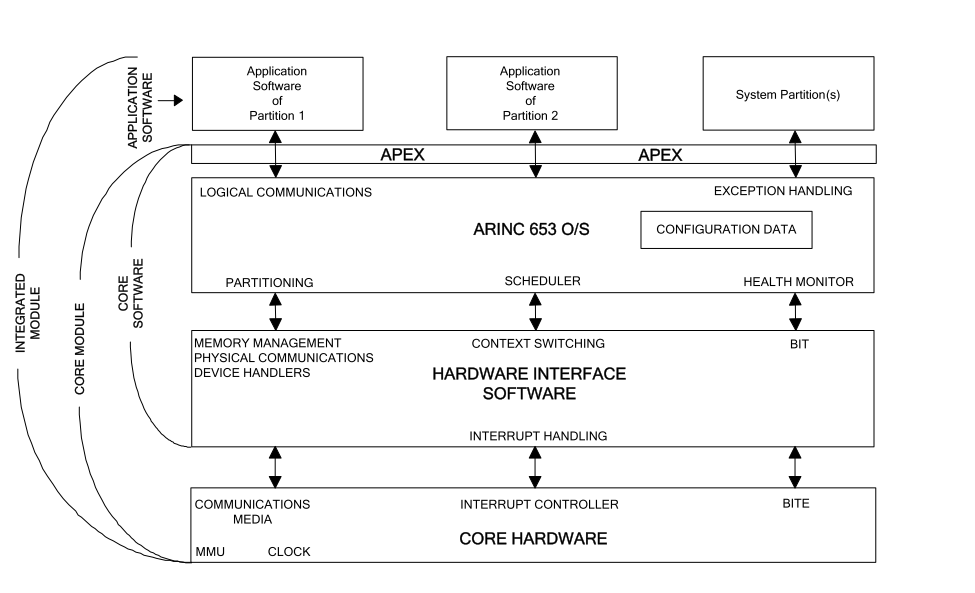
\includegraphics[scale=0.3]{resources/arinc653-architecture.png}
        \end{figure}
    \end{frame}
    \begin{frame}
        \frametitle{\textit{Primary-Backup Scheduling}}
        \begin{itemize}
            \item Metode \textit{scheduling} proses yang menjamin \textit{fault-tolerancy}.
            \item Pada kondisi normal, \textit{scheduler} akan melakukan \textit{scheduling} untuk proses \textit{primary}.
            \item Proses \textit{primary} gagal $\implies$ proses \textit{backup} menggantikan.
        \end{itemize}
    \end{frame}
    \begin{frame}
        \frametitle{\textit{Primary-Backup Scheduling} --- \textit{Process List}}
        \begin{figure}[htbp]
            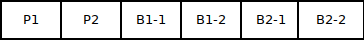
\includegraphics[scale=0.5]{resources/process_list.png}
            \caption*{\textit{Process List}}
            \\[25pt]
            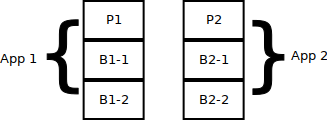
\includegraphics[scale=0.5]{resources/process_list_desc.png}
            \caption*{Aplikasi pada \textit{Process List}}
        \end{figure}
    \end{frame}
    \begin{frame}
        \frametitle{\textit{Primary-Backup Scheduling} --- \textit{Normal Scheduling}}
        \begin{figure}[htbp]
            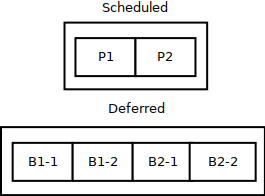
\includegraphics[scale=0.7]{resources/schedule_normal.png}
        \end{figure}
    \end{frame}
    \begin{frame}
        \frametitle{\textit{Primary-Backup Scheduling} --- \textit{Fault}}
        \begin{figure}[htbp]
            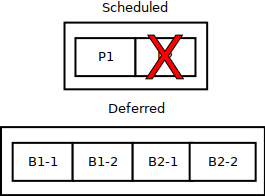
\includegraphics[scale=0.7]{resources/fault.png}
        \end{figure}
    \end{frame}
    \begin{frame}
        \frametitle{\textit{Primary-Backup Scheduling} --- \textit{On-Fault Scheduling}}
        \begin{figure}[htbp]
            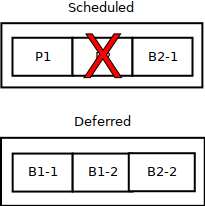
\includegraphics[scale=0.7]{resources/schedule_onfault.png}
        \end{figure}
    \end{frame}
    \begin{frame}
        \frametitle{Xen}
        \begin{itemize}
            \item Hypervisor yang memanajemeni \textit{virtual machine} (pada Xen disebut sebagai \textit{domain}).
            \item Setiap \textit{virtual machine} memiliki lingkungan terisolasi (mesin fisik menjadi terpartisi).
            \item Dapat digunakan untuk memodelkan partisi pada spesifikasi ARINC 653.
            \item Free \& Open Source $\implies$ mudah melakukan \textit{customization}:
                \begin{itemize}
                    \item Memiliki \textit{interface} untuk membuat \textit{scheduler}
                    \item Memiliki \textit{interface} untuk membuat konfigurasi \textit{domain}
                \end{itemize}
            \item Produk serupa:
                \begin{itemize}
                    \item VMWare
                    \item VirtualBox
                \end{itemize}
        \end{itemize}
    \end{frame}
    \begin{frame}
        \frametitle{Xen ARINC 653}
        \begin{itemize}
            \item Prototipe sistem yang memenuhi standar ARINC 653.
            \item Dikembangkan diatas Xen  $\implies$ memiliki karakteristik dan keuntungan Xen.
        \end{itemize}
    \end{frame}
    \section{Rumusan Masalah \& Tujuan}
    \begin{frame}
        \frametitle{Rumusan Masalah \& Tujuan}
        \begin{itemize}
            \item Belum ada implementasi maupun penelitian tentang \textit{primary-backup scheduling} pada sistem yang memenuhi standar ARINC 653.
            \item Penelitian ini akan menjawab permasalahan mengenai:
                \begin{itemize}
                    \item Implementasi \textit{primary-backup scheduling} pada Xen ARINC 653
                    \item Pengujian \textit{scheduling} pada Xen ARINC 653
                    \item ARINC 653 + \textit{primary-backup scheduling} $\implies$ lebih \textit{fault-tolerant}
                    \item Kinerja ARINC 653 + \textit{primary-backup scheduling} vs normal
                \end{itemize}
        \end{itemize}
    \end{frame}
    \section{Analisis}
    \begin{frame}
        \frametitle{Xen ARINC 653 --- \textit{Scheduling}}
        \begin{itemize}
            \item Memodelkan partisi dengan menggunakan \textit{domain}
            \item Menggunakan \textit{major time frame} (didapat dari faktor persekutuan terbesar \textit{deadline} seluruh partisi)
            \item Aplikasi akan meminta \textit{slot} pada \textit{major time frame}
            \item Diimplementasikan pada \textit{file} 'xen/common/sched\_arinc653.c'
        \end{itemize}
    \end{frame}
    \begin{frame}
        \frametitle{Xen ARINC 653 --- Contoh Partisi}
        \begin{figure}[htbp]
            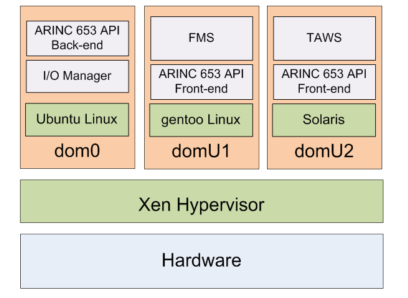
\includegraphics[scale=0.4]{resources/xen-arinc653-partitions.png}
            \caption*{Contoh partisi yang akan dijalankan}
        \end{figure}
    \end{frame}
    \begin{frame}
        \frametitle{Xen ARINC 653 --- Contoh \textit{Scheduling}}
        \begin{figure}[htbp]
            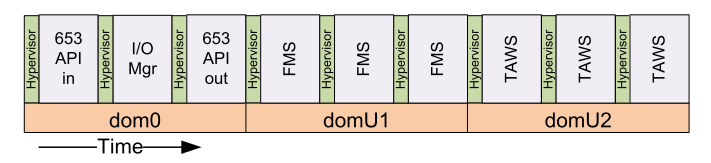
\includegraphics[scale=0.4]{resources/xen-arinc653-partition-schedule.png}
            \caption*{\textit{Scheduling} pada Xen ARINC 653}
        \end{figure}
    \end{frame}
    \begin{frame}
        \frametitle{Implementasi \textit{Primary-Backup} Scheduling}
        \begin{itemize}
            \item Penentuan Jenis \textit{Partisi} (\textit{primary}/\textit{backup})
                \begin{itemize}
                    \item \textit{Hardcode} nama
                    \item Menambahkan \textit{property} pada saat konfigurasi \textit{domain}
                \end{itemize}
            \item Pendeteksian Kegagalan
                \begin{itemize}
                    \item Komunikasi kepada \textit{domain} utama/dom0 (menggunakan \textit{shared memory}, XenStore)
                    \item Komunikasi kepada \textit{hypervisor} (menggunakan \textit{hypercall})
                \end{itemize}
        \end{itemize}
    \end{frame}
    \begin{frame}
        \frametitle{Evaluasi}
        \begin{itemize}
            \item \textit{Stress-testing}
                \begin{enumerate}
                    \item Aplikasi akan bekerja bersamaan dengan aplikasi lain.
                    \item Hitung persentase \textit{deadline} yang terpenuhi
                \end{enumerate}
            \item \textit{Fault-injection}
                \begin{enumerate}
                    \item Aplikasi akan diberikan \textit{request}.
                    \item Aplikasi akan memiliki kemungkinan untuk mengalami \textit{fault}.
                    \item Hitung persentase aplikasi tidak mengalami \textit{fault}.
                \end{enumerate}
        \end{itemize}
    \end{frame}
    \begin{frame}
        \Huge Terima Kasih
    \end{frame}
    \begin{frame}
        \frametitle{F.A.Q}
        \begin{itemize}
            \item \textit{Hypervisor} --- \textit{Supervisor} dari \textit{supervisor} (kernel), \textit{hyper} $>$ \textit{super}
            \item dom0 --- \textit{Domain} yang melakukan manajemen \textit{domain}/\textit{virtual machine} lain
        \end{itemize}
    \end{frame}
\end{document}
